\section{Figures}\label{sec:figures}

\subsection{Double Pendulum Details}\label{subsec:double-pendulum-details}
\begin{figure}[H]
    \centering
    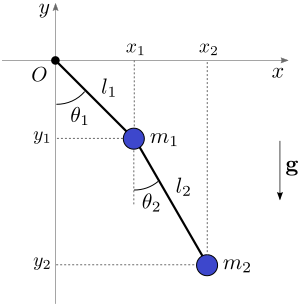
\includegraphics[scale=1]{double-pendulum.png}
    \caption{A visualization of a double pendulum}
    \label{fig:1}
\end{figure}

\subsection{Results from the first set of initial conditions}\label{subsec:results-from-the-first-set-of-initial-conditions}
\begin{figure}[H]
    \centering
    \begin{subfigure}[b]{0.49\textwidth}
        \centering
        \includegraphics[width=\textwidth]{initial-conditions-a/theta_2 vs theta_1.png}
        \caption{$\theta_2$ vs $\theta_1$.}
        \label{fig:2a}
    \end{subfigure}
    \hfill
    \begin{subfigure}[b]{0.49\textwidth}
        \centering
        \includegraphics[width=\textwidth]{initial-conditions-a/omega_2 vs omega_1.png}
        \caption{$\omega_2$ vs $\omega_1$.}
        \label{fig:2b}
    \end{subfigure}
    \hfill
    \begin{subfigure}[b]{0.49\textwidth}
        \centering
        \includegraphics[width=\textwidth]{initial-conditions-a/Angular Positions vs Time.png}
        \caption{$\theta_1, \theta_2$ vs time.}
        \label{fig:2c}
    \end{subfigure}
    \hfill
    \begin{subfigure}[b]{0.49\textwidth}
        \centering
        \includegraphics[width=\textwidth]{initial-conditions-a/Angular Velocities vs Time.png}
        \caption{$\omega_1, \omega_2$ vs time.}
        \label{fig:2d}
    \end{subfigure}
    \hfill
    \begin{subfigure}[b]{0.49\textwidth}
        \centering
        \includegraphics[width=\textwidth]{initial-conditions-a/Energies vs Time.png}
        \caption{Potential, Kinetic, and Total Energies vs time.}
        \label{fig:2e}
    \end{subfigure}
    \caption{Solving the system from $t_1 = 0\text{ s}$ to $t_2 = 10\text{ s}$ where $m_1 = 1\text{ kg}$, $m_2 = 1\text{ kg}$, $l_1 = 1\text{ m}$, $l_2 = 1\text{ m}$, $\theta_{1,0} = 45^\circ$, $\theta_{2,0} = 0^\circ$, $\omega_{1,0} = 0^\circ\text{/s}$, $\omega_{2,0} = 0^\circ\text{/s}$.}
    \label{fig:2}
\end{figure}

\subsection{Results from the second set of initial conditions}\label{subsec:results-from-the-second-set-of-initial-conditions}
\begin{figure}[H]
    \centering
    \begin{subfigure}[b]{0.49\textwidth}
        \centering
        \includegraphics[width=\textwidth]{initial-conditions-b/theta_2 vs theta_1.png}
        \caption{$\theta_2$ vs $\theta_1$.}
        \label{fig:3a}
    \end{subfigure}
    \hfill
    \begin{subfigure}[b]{0.49\textwidth}
        \centering
        \includegraphics[width=\textwidth]{initial-conditions-b/omega_2 vs omega_1.png}
        \caption{$\omega_2$ vs $\omega_1$.}
        \label{fig:3b}
    \end{subfigure}
    \hfill
    \begin{subfigure}[b]{0.49\textwidth}
        \centering
        \includegraphics[width=\textwidth]{initial-conditions-b/Angular Positions vs Time.png}
        \caption{$\theta_1, \theta_2$ vs time.}
        \label{fig:3c}
    \end{subfigure}
    \hfill
    \begin{subfigure}[b]{0.49\textwidth}
        \centering
        \includegraphics[width=\textwidth]{initial-conditions-b/Angular Velocities vs Time.png}
        \caption{$\omega_1, \omega_2$ vs time.}
        \label{fig:3d}
    \end{subfigure}
    \hfill
    \begin{subfigure}[b]{0.49\textwidth}
        \centering
        \includegraphics[width=\textwidth]{initial-conditions-b/Energies vs Time.png}
        \caption{Potential, Kinetic, and Total Energies vs time.}
        \label{fig:3e}
    \end{subfigure}
    \caption{Solving the system from $t_1 = 0\text{ s}$ to $t_2 = 10\text{ s}$ with the same intial conditions from \myref[Figure]{fig:2} but with $\theta_{2,0} = 0^\circ$ instead.}
    \label{fig:3}
\end{figure}
